% ==============================================================
% SECCIÓN 3: ADALINE — APRENDIZAJE DE BEMF
% ==============================================================

% --- Slide 8: ¿Qué es ADALINE? ---
\begin{frame}{ADALINE: Adaptive Linear Neuron (Widrow-Hoff, 1960)}
    Red neuronal de \textbf{una sola capa, sin no-linealidad}, con base de entrada de Fourier:
    
    \begin{equation}
        \hat{s}_\alpha(\theta) = \mathbf{w}_\alpha^T \mathbf{x}(\theta) = \sum_{n=1}^{H} \left[ w_n^c \cos(n\theta) + w_n^s \sin(n\theta) \right]
    \end{equation}
    
    donde el vector de regresores es:
    \begin{equation}
        \mathbf{x}(\theta) = \begin{bmatrix} \cos\theta & \sin\theta & \cos 2\theta & \sin 2\theta & \cdots & \cos H\theta & \sin H\theta \end{bmatrix}^T \in \mathbb{R}^{2H}
    \end{equation}
    
    \begin{itemize}
        \item Con $H = 10$ armónicos: \textbf{40 parámetros totales} (20 por eje $\alpha, \beta$).
        \item Los pesos $w_n^c, w_n^s$ \textbf{son los coeficientes de Fourier} de la BEMF.
        \item Interpretación física directa: $|w_5| = $ amplitud del 5to armónico.
    \end{itemize}
\end{frame}

% --- Slide 9: ¿Por qué ADALINE y no una NN profunda? ---
\begin{frame}{¿Por Qué ADALINE y No una Red Neuronal Profunda?}
    \begin{columns}[T]
    \begin{column}{0.48\textwidth}
        \begin{block}{Red Profunda (BEMFNet)}
            \begin{itemize}
                \item 4 capas ocultas (64--128 neuronas)
                \item $\sim$25,000 parámetros
                \item Entrenamiento: 300 epochs, $\sim$30 s
                \item Backpropagation: $O(N_{\text{params}})$ por paso
                \item Mínimo local (no convexo)
                \item Pesos: caja negra
            \end{itemize}
        \end{block}
    \end{column}
    \begin{column}{0.48\textwidth}
        \begin{exampleblock}{ADALINE + Fourier}
            \begin{itemize}
                \item 1 capa, sin activación
                \item \textbf{40 parámetros}
                \item Entrenamiento: pseudoinversa, $\sim$12 ms
                \item LMS online: $O(2H)$ por paso
                \item \textbf{Óptimo global} (problema convexo)
                \item Pesos = espectro de Fourier
            \end{itemize}
        \end{exampleblock}
    \end{column}
    \end{columns}
    
    \vspace{0.4cm}
    
    \begin{center}
        \fcolorbox{ForestGreen}{green!5}{\parbox{0.85\textwidth}{\centering
            La BEMF es una \textbf{función periódica de $\theta$} $\rightarrow$ la serie de Fourier es su representación \textbf{natural y óptima}.\\
            Usar una NN profunda para esto es \textit{usar un aproximador universal cuando existe la solución exacta}.
        }}
    \end{center}
\end{frame}

% --- Slide 10: Entrenamiento offline ---
\begin{frame}{Fase 0: Entrenamiento Offline (Pseudoinversa)}
    Dado el dataset $\{(\theta_k, s_{\alpha,k}, s_{\beta,k})\}_{k=1}^{N}$, construimos:
    \begin{equation}
        \mathbf{X} = \begin{bmatrix} \mathbf{x}(\theta_1)^T \\ \vdots \\ \mathbf{x}(\theta_N)^T \end{bmatrix} \in \mathbb{R}^{N \times 2H}, \qquad
        \mathbf{W}^* = (\mathbf{X}^T\mathbf{X})^{-1}\mathbf{X}^T \mathbf{S} = \mathbf{X}^\dagger \mathbf{S}
    \end{equation}
    
    \begin{columns}[T]
    \begin{column}{0.42\textwidth}
        \centering
        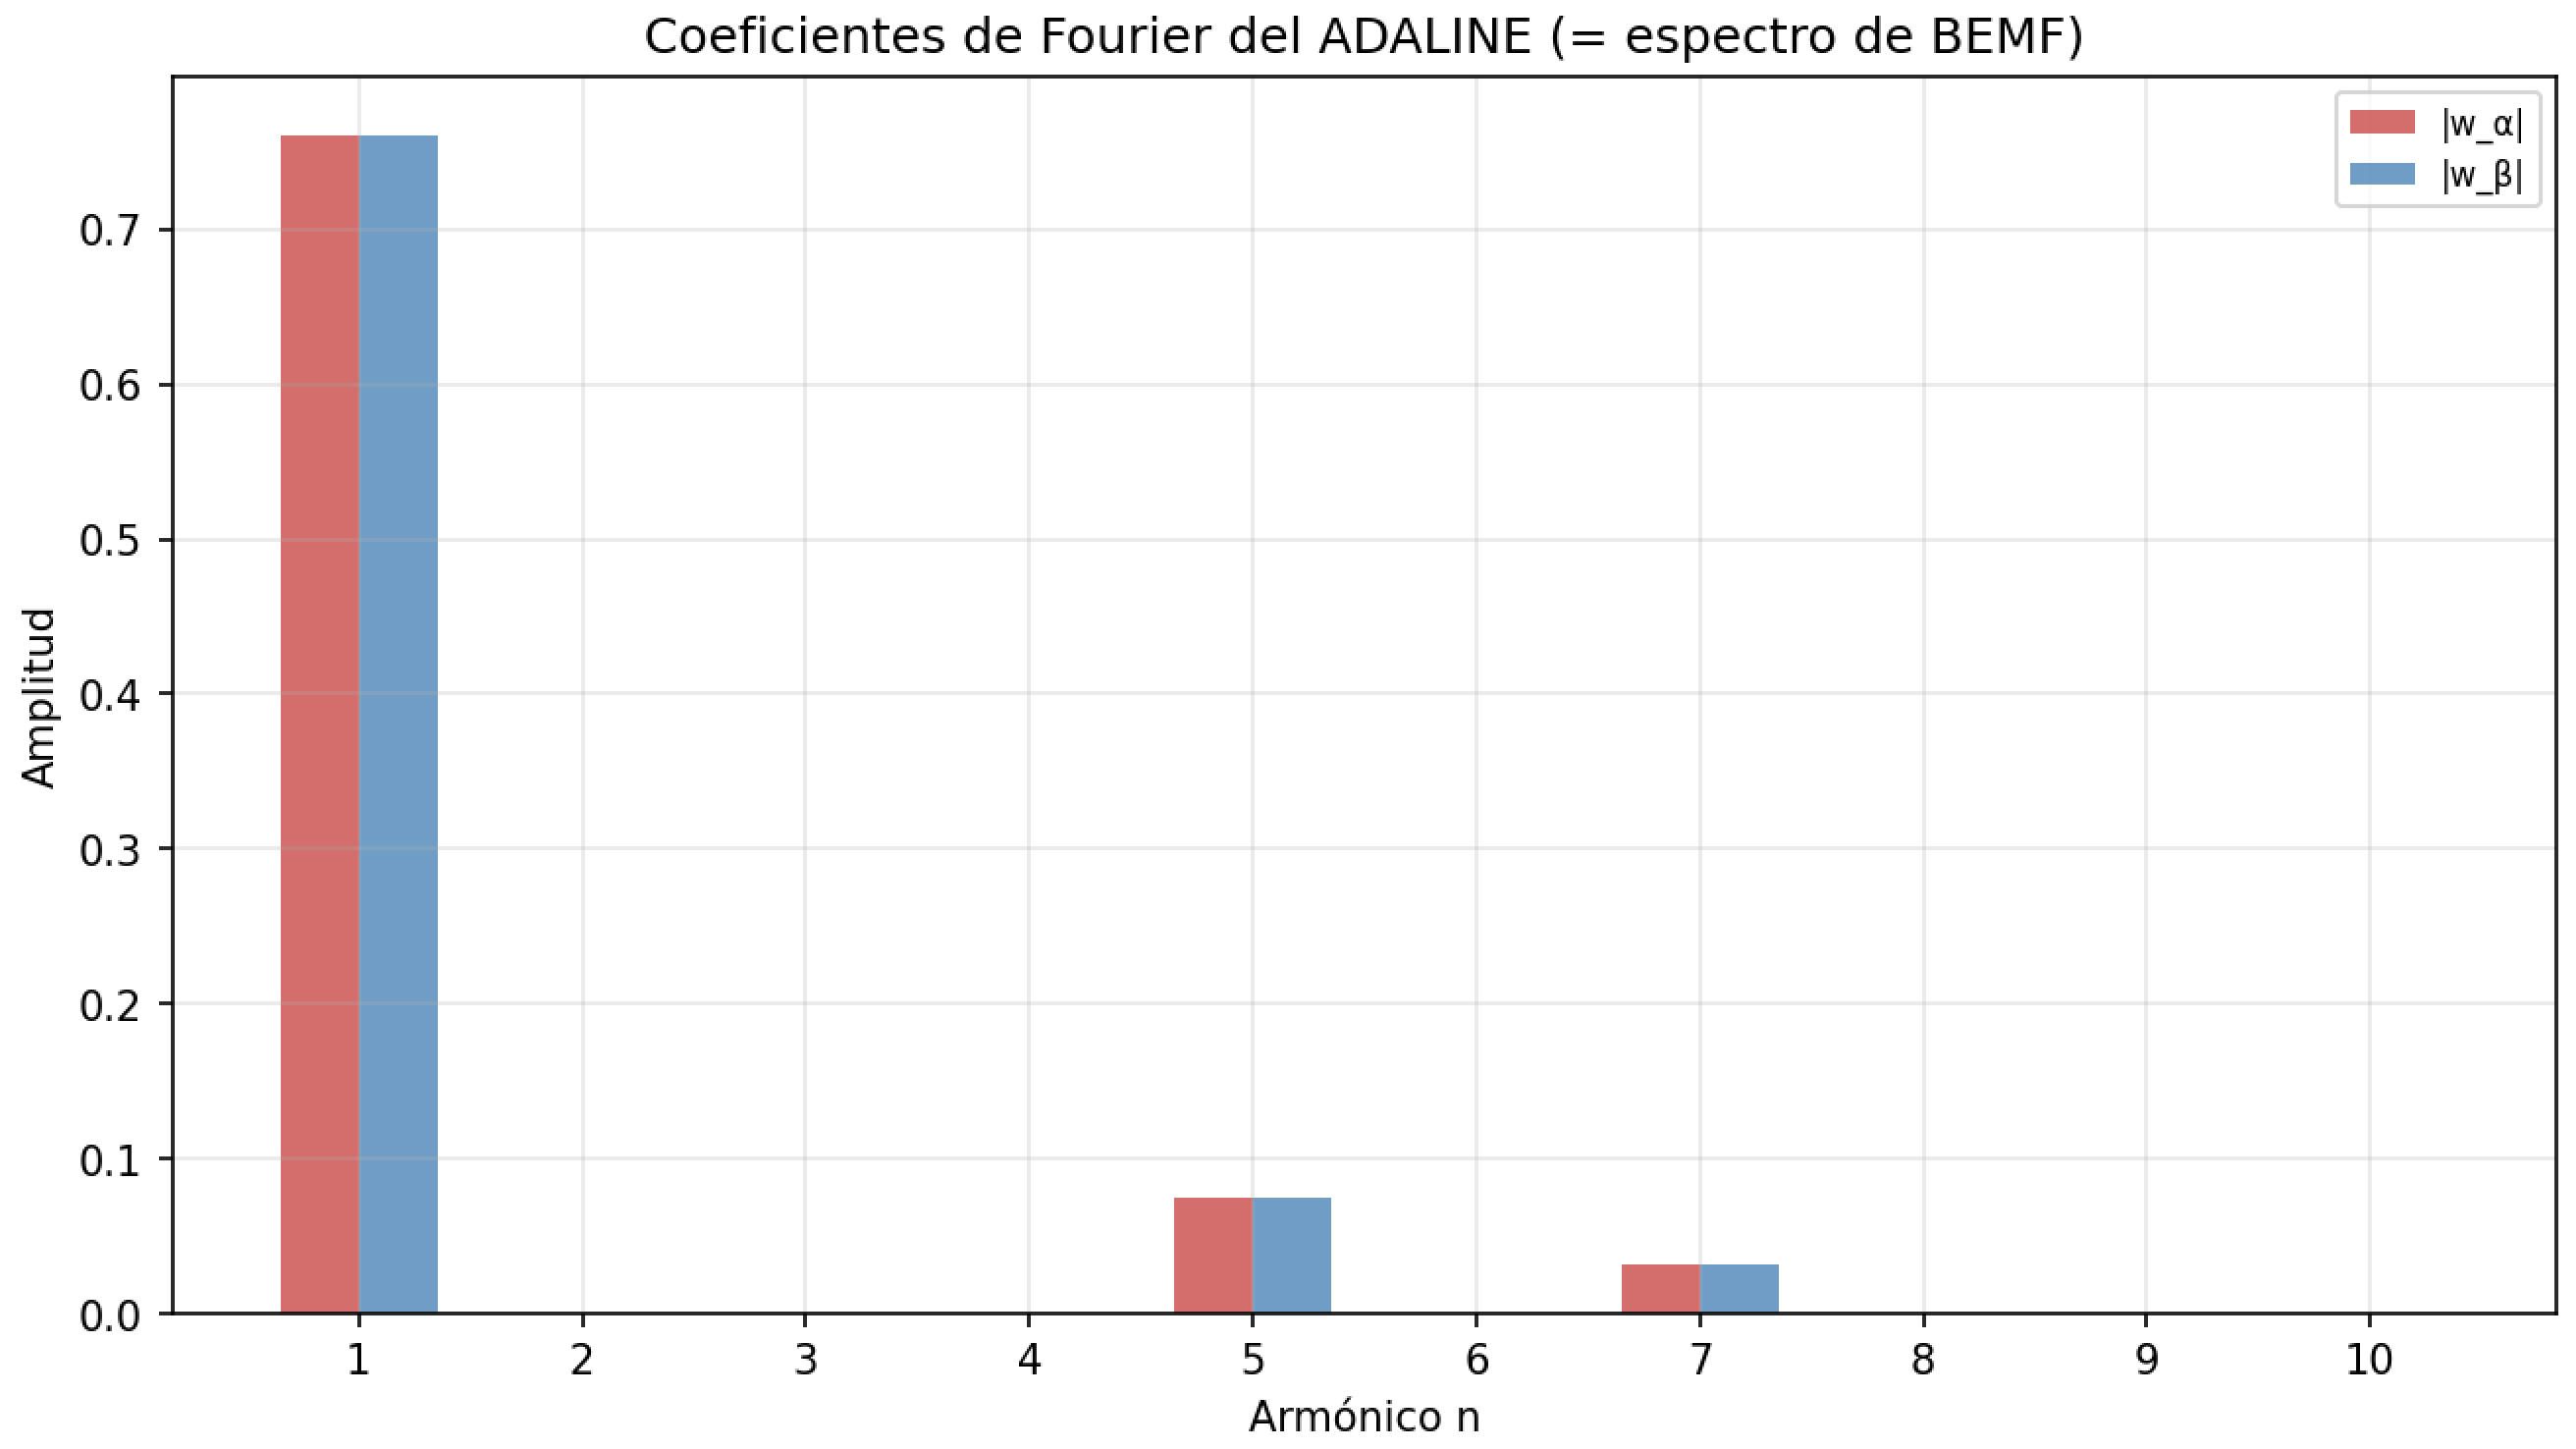
\includegraphics[width=0.99\linewidth]{fig/adaline_fourier_coeffs.png}
        {\footnotesize Coeficientes de fourier por armónico}
    \end{column}
    \begin{column}{0.42\textwidth}
        \centering
        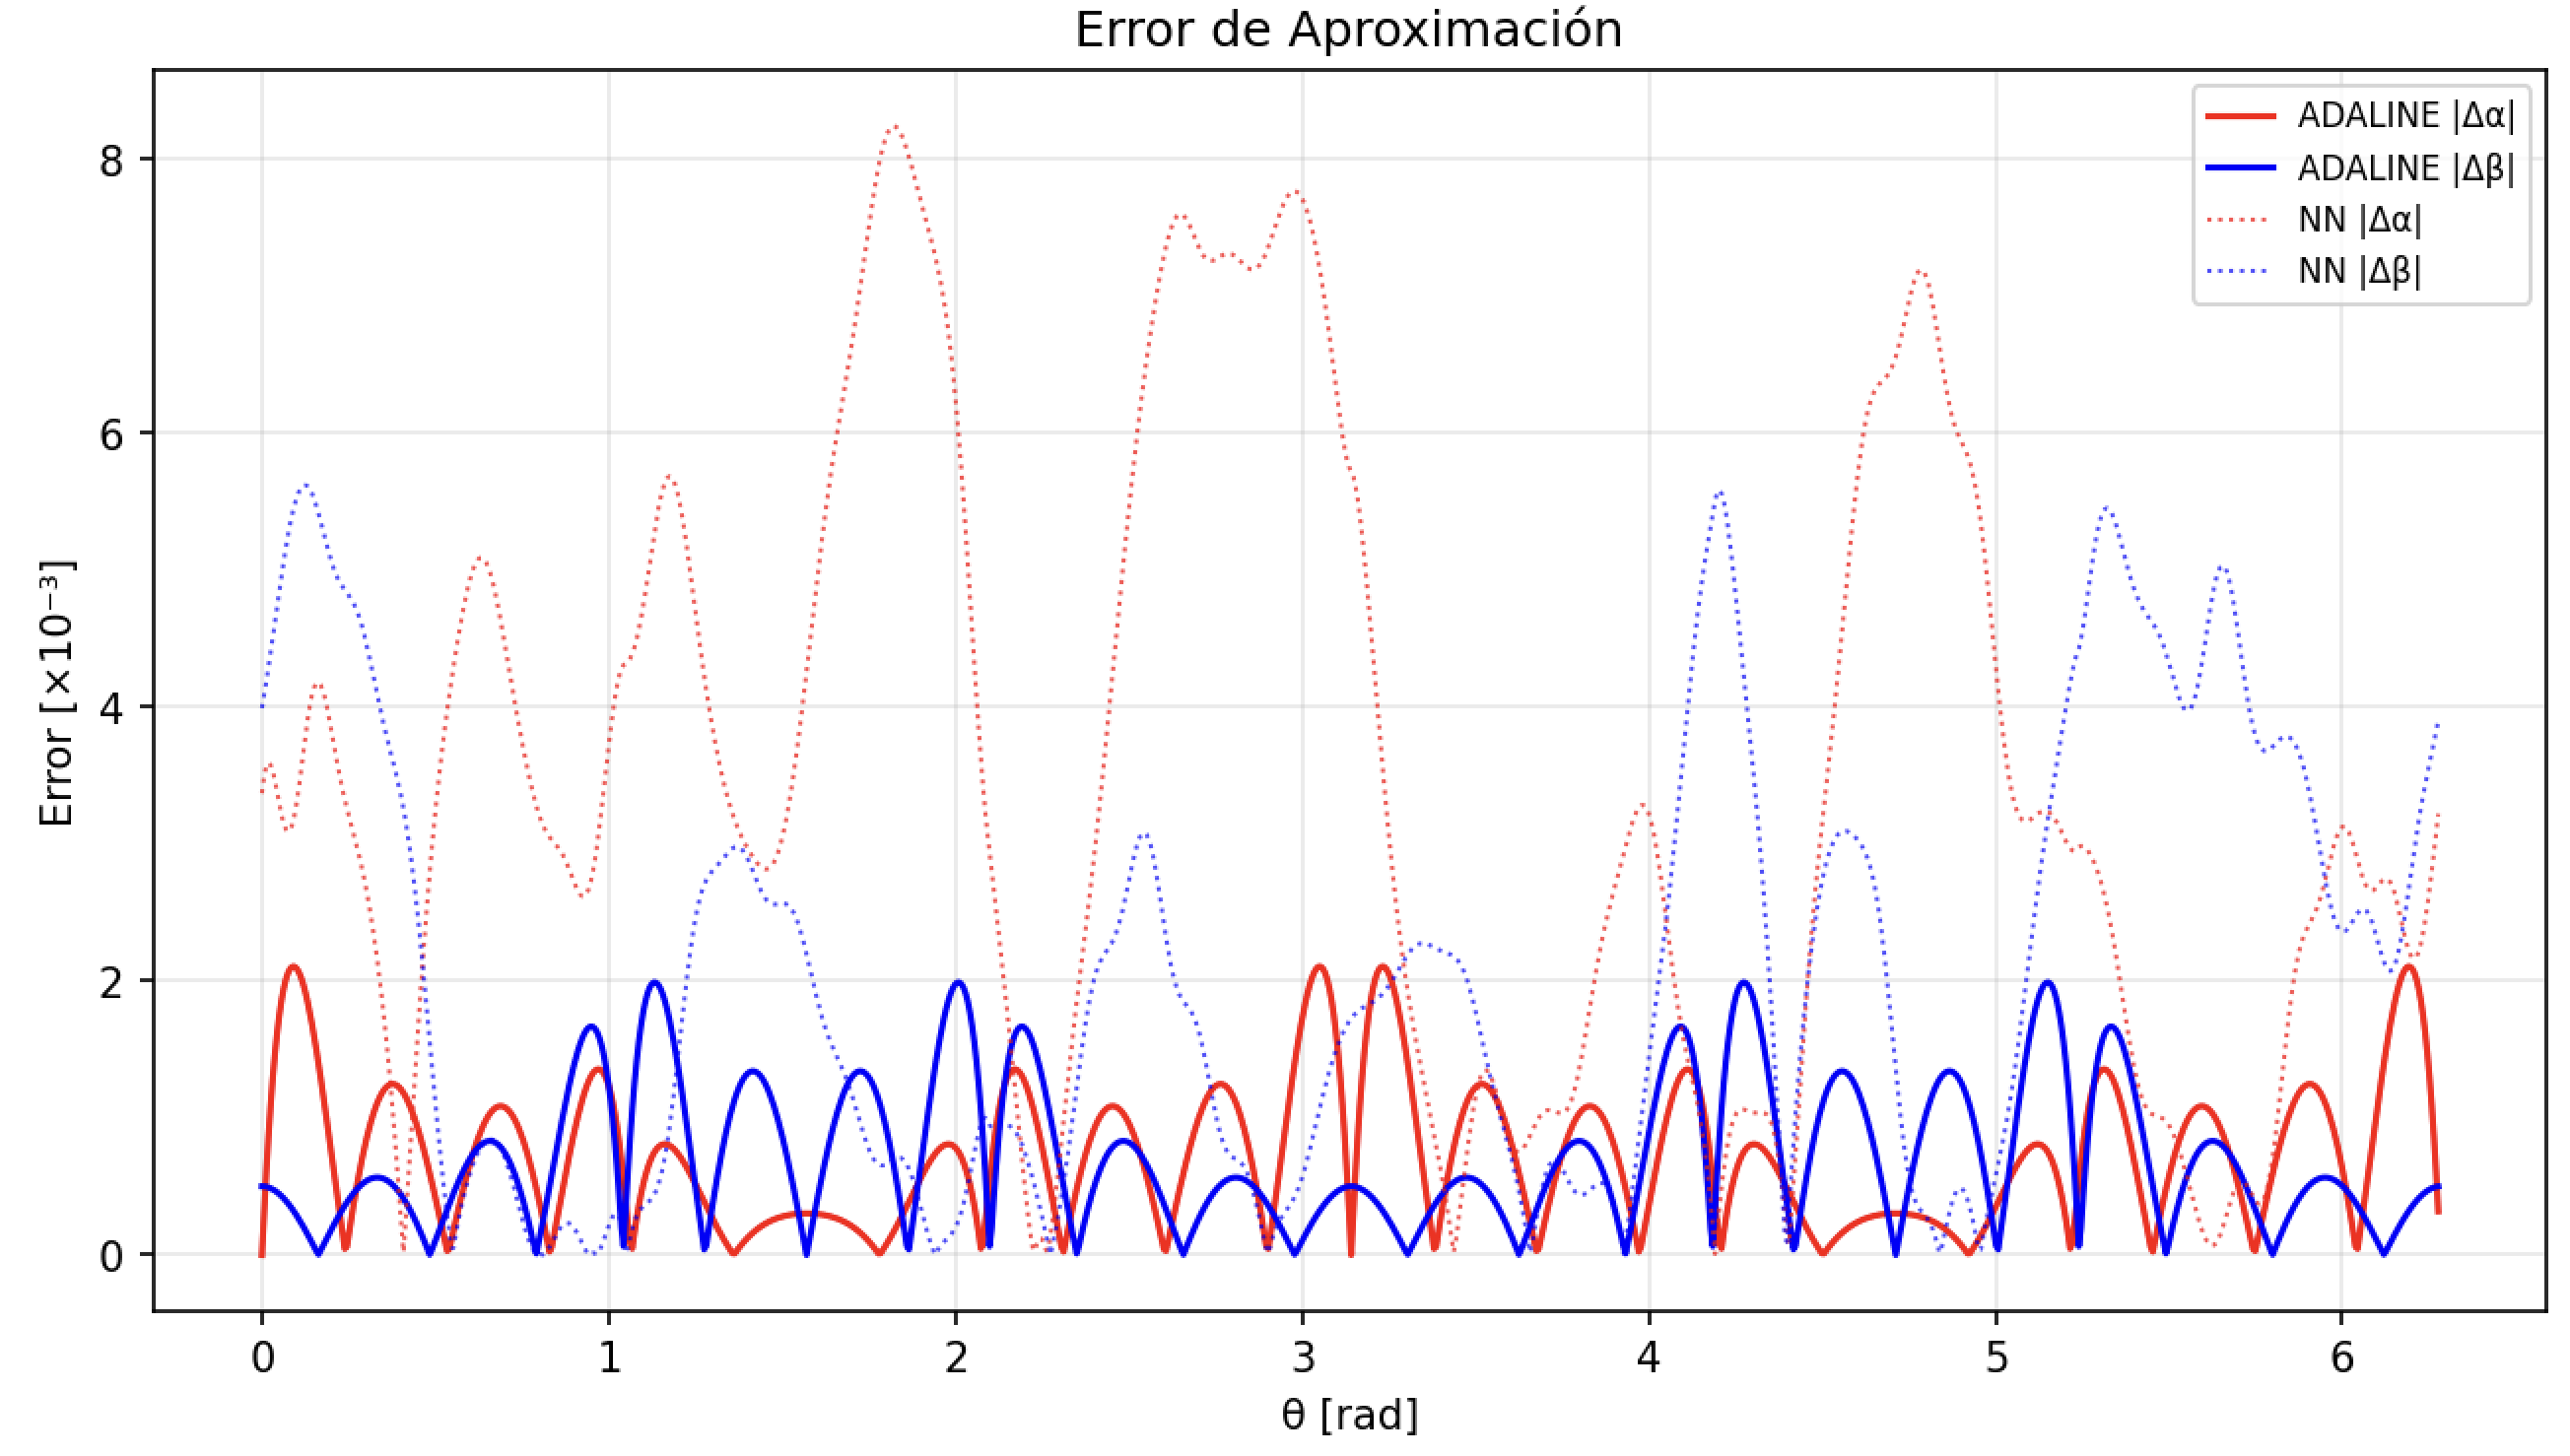
\includegraphics[width=0.99\linewidth]{fig/adaline_vs_nn_alpha.png}
        {\footnotesize ADALINE vs NN}
    \end{column}
    \end{columns}
\end{frame}

% --- Slide 11: ADALINE online con LMS ---
\begin{frame}{Fase 1: Aprendizaje Online con LMS}
    \textbf{Ley de actualización} (Least Mean Squares):
    \begin{equation}
        \mathbf{w}(k+1) = \mathbf{w}(k) + \mu \cdot \underbrace{\left[s_{\text{obs}}(k) - \mathbf{w}^T(k)\mathbf{x}(\theta_k)\right]}_{\text{error de estimación } \epsilon(k)} \cdot \mathbf{x}(\theta_k)
    \end{equation}
    
    \vspace{0.2cm}
    
    \begin{columns}[T]
    \begin{column}{0.48\textwidth}
        \textbf{Propiedades clave:}
        \begin{itemize}
            \item \textbf{Convergencia:} $0 < \mu < 4$ (base ortogonal $\rightarrow$ $\lambda_{\max} = 1/2$)
            \item \textbf{Velocidad:} $\tau \approx 1/\mu$ pasos $\approx$ 1--2 rev eléctricas
            \item \textbf{Misadjustment:} $M \approx \mu H$ (residuo en régimen permanente)
            \item \textbf{Costo:} 1 producto punto por paso ($\sim$\textbf{microsegundos} en DSP)
        \end{itemize}
    \end{column}
    \begin{column}{0.48\textwidth}
        \textbf{¿Qué significa esto?}
        \begin{itemize}
            \item El motor se \textbf{auto-calibra} en $\sim$50 ms
            \item No necesita datos previos del fabricante
            \item Se adapta a cambios térmicos, envejecimiento, tolerancias de fabricación
            \item \textbf{Implementable en DSP} (TMS320F28xxx) sin modificaciones de hardware
        \end{itemize}
    \end{column}
    \end{columns}
\end{frame}

% --- Slide 12: Idoneidad del ADALINE ---
\begin{frame}{¿Por Qué ADALINE es \textit{Idóneo} para Este Problema?}
    
    Tres razones estructurales (no cosméticas):
    
    \vspace{0.3cm}
    
    \begin{enumerate}
        \item \textbf{La BEMF es periódica en $\theta$} $\rightarrow$ la serie de Fourier es completa y ortogonal para funciones periódicas. No hay pérdida de generalidad al truncar a $H$ armónicos si la energía espectral por encima de $H$ es despreciable.
        
        \vspace{0.2cm}
        
        \item \textbf{La base $\{\cos n\theta, \sin n\theta\}$ tiene $\|\mathbf{x}\|^2 = H$ constante} $\rightarrow$ todos los modos convergen a la misma velocidad (no hay \textit{eigenvalue spread}). El LMS es \textbf{óptimamente condicionado} para esta base.
        
        \vspace{0.2cm}
        
        \item \textbf{Los pesos son directamente los coeficientes de Fourier} $\rightarrow$ se puede inspeccionar \textit{qué armónicos tiene el motor} mirando $|w_n|$. Además, estos pesos son la \textbf{inicialización natural} para un controlador repetitivo que necesita conocer el espectro del disturbio.
    \end{enumerate}
    
    \vspace{0.3cm}
    
    \begin{center}
        \small
        $\underbrace{\text{ADALINE offline}}_{\text{Fase 0: modelo base}}
        \;\xrightarrow{\text{LMS}}\;
        \underbrace{\text{ADALINE online}}_{\text{Fase 1: auto-calibración}}
        \;\xrightarrow{\text{pesos} \rightarrow \text{espectro}}\;
        \underbrace{\text{Control Repetitivo}}_{\text{Fase 3: rechazo periódico}}$
    \end{center}
\end{frame}